\chapter{Conics}

A conic section, a conic, or a quadratic curve is a curve obtained from a cone's surface
intersecting a plane.

\section{Dandelin Spheres}

Germinal Pierre Dendelin, a 19th century French-Belgian Professor, discovered this beautiful
proof to demonstrate that any plane that cuts through a right circular cone produces a
quadratic curve.

\begin{theorem}
  When a plane intersects a right circular cone, the curve produced will either be an ellipse,
  a parabola or a hyperbola.
\end{theorem}

\begin{proof}
  Place a sphere tangent to the intersecting plane $\pi$ and the cone such that it touches the
  plane at $F$, and the cone in a circle $C$ with centre $O$ that lies on a horizontal plane
  $\epsilon$. \footnote{Assuming such sphere exists.}

  Take an aribtrary point $P$ on the curve $Q$, and extend the line $VP$ from the vertex $V$
  of the cone to meet $C$ at point $L$. Let $D$ be the point on the intersection on the planes
  $\pi$ and $\epsilon$ such that $PD$ is perpendicular to the line of intersection. (If the
  planes do not intersect, $Q$ will be a circle)

  Drop a perpendicular $PM$ on $OL$ such that $\triangle PML$ and $\triangle PMD$ are both
  right angled. Denote $\angle PLM$ as $\alpha$, and $\angle PDM$ as $\beta$.

  From the triangles  $\triangle PML$ and $\triangle PMD$
    \begin{eqnarray*}
    \sin{\alpha}&=&\frac{PM}{PD}\\ 
    \quad \textrm{and} \quad \sin{\beta}&=&\frac{PM}{PL}\\
    \quad \textrm{i.e.} \quad \frac{PL}{PD}&=&\frac{\sin{\alpha}}{\sin{\beta}}
  \end{eqnarray*}

  \begin{figure}[H]
    \center
    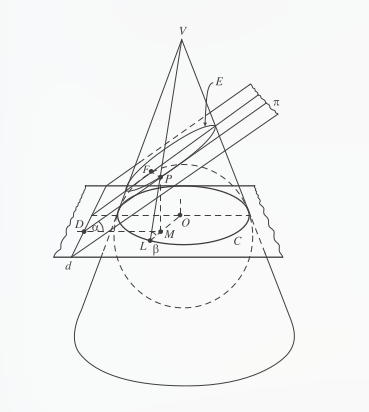
\includegraphics[width=0.85\linewidth]{dandelin.png}
    \caption{When $0<\alpha<\beta<\frac{\pi}{2}$}
  \end{figure}


 
  Since $PL$ and $PF$ are both tangents from $P$ to the sphere, $PF=PL$. Therfore,
  \[\frac{PF}{PD}=\frac{\sin{\alpha}}{\sin{\beta}}\]
  i.e. $PF=e\cdot PD$, where $e=\sin{\alpha}/\sin{\beta}$\\
  It follows from the focus - directrix definition that $Q$ will be an ellipse if
  $\alpha<\beta$, a parabola if $\alpha=\beta$, or a hyperbola if $\alpha>\beta$.
\end{proof}
Proof adapted from \cite{brannan} with modifications to generalize it for all conics.

\section{Group Laws on Conics}

Consider a conic section $C$ and a point $O \in C$ For any $P,Q \in C$,define a binary
operation $\oplus :C \times C \rightarrow C$ by $P \oplus Q = R$, where $R$ is such that $l_{PQ} \Vert l_{OR}$.

\begin{theorem}
Set of points of $C$ forms a group $G(C)$ under the binary operation $\oplus$, with $O$ as the
identity element.
\end{theorem}

\begin{proof}\textbf{Closure:} The line through $O$ parallel to $l_{PQ}$ necessarily meets $C$
  again, (counting algebraic multiplicities) since for any quadratic equation with real 
  coeffecients, if one of the roots is real, the other one must be real too. \vspace{10pt}

  \textbf{Existence of Identity Element:} The point $O$ serves as the identity element. \vspace{0pt}

  \textbf{Existence of Inverse:} Constructively, when $Q$ is such that the line parellel to
  $l_{PQ}$ that passes through $O$ is tangent to the conic, i.e when $R=O$, we get
  $P\oplus Q=O$. So, $Q$ serves as the inverse of $P$. \vspace{10pt}

  \textbf{Associativity:} To prove associativity, we'll find algebraic formula for $P\oplus Q$
  for standard conics, i.e for the circle $x^2+y^2=1$, for the parabloa $y=x^2$, and for the
  hyperbola $xy=1$. In the next chapter, we'll prove that any ellipse, hyperbola or parabola
  is affine congruent to its standard form. This result will generalize the result to all
  conics. The following formulae will be valid for any fields with non-two charecteristic.

  Let the point $P$ be $(p_1,p_2)$, $Q$ be $(q_1,q_2)$, $O$ be $(o_1,o_2)$, and $R$ be
  $(r_1,r_2)$, and let the slope of the line $l_{PQ}$ be $\lambda=q_2-p_2/q_1-p_1$, assuming
  $P\not=Q$, since associativity would be trivial then. Let $\ell$ be the line through $O$
  with slope $\lambda$. The coordinates of $R$ will satisfy
  $\lambda=\frac{r_2-o_2}{r_1-o_2}=\frac{q_2-p_2}{q_1-p_1}$,
  $\Rightarrow$ $r_2=o_2+\mu(q_2-p_2)$ and $r_1=o_1+\mu(q_1-p_1)$ for some $\mu\in\mathbb{F}$.

  \begin{itemize}
    \item[(i)]{\textbf{Circle}\\
        Without loss of generality, let $O=(1,0)$. Since $R$ also lies on $C$,
        $r_1^2+r_2^2=1$. i.e.

        \begin{eqnarray*}
          &&(1+\mu(q_1-p_1))^2+(0+\mu(q_2-p_2))^2=1\\
          \Rightarrow && \mu(\mu(q_1-p_1)^2+\mu(q_2-p_2)^2+2(q_1-p_1))=0\\
          \Rightarrow && \mu=0\text{ or }\mu=-\frac{2(q_1-p_1)}{(q_1-p_1)^2+(q_2-p_2)^2}
        \end{eqnarray*}

        We assume that $(q_1-p_1)^2+(q_2-p_2)^2\not=0$. Because if it was so,

        \begin{eqnarray*}
          &&q_1^2+p_1^2-2q_1p_1+q_2^2+p_2^2-2p_2q_2=0\\
          \Rightarrow&&1-p_1q_1-p_2q_2=0\\
          \Rightarrow&&p_1^2q_1^2=1+p_2^2q_2^2-2p_2q_2\\
          \Rightarrow&&p_1^2q_1^2=1+(1-p_1^2)(1-q_1^2)-2p_2q_2\\
          \Rightarrow&&0=2-p_1^2-q_1^2-2p_2q_2\\
          \Rightarrow&&(p_2-q_2)^2=0\\
          \Rightarrow&&p_2=q_2\text{ and similarly, }p_1=q_1
        \end{eqnarray*}

        Which is when $P=Q$, which we have assummed not to be true.

        \begin{figure}[H]
          \center
          \begin{tikzpicture}
            \tkzDefPoint(0,0){C}
            \tkzDefPoint(3,0){O}
            \tkzDefPoint(0,3){P}
            \tkzDefPoint(-3,0){Q}
            \tkzDefPoint(0,-3){R}
            \tkzDrawPoints[fill=black](O,P,Q,R)
            \tkzDrawLine[<->, line width=0.5, add=0.2 and 0.2](P,Q)
            \tkzDrawLine[<->, line width=0.5, add=0.2 and 0.2](O,R)
            \tkzDrawCircle[color=black, line width=0.5](C,O)
            \tkzLabelPoints[below right](O)
            \tkzLabelPoints[below right](R)
            \tkzLabelPoints[above left](P)
            \tkzLabelPoints[above left](Q)
          \end{tikzpicture}
          \caption{$R = P \oplus Q$ when $C$ is a circle.}
        \end{figure}

        The $\mu=0$ solution corresponds to $O$. Considering the other solution,

        \begin{eqnarray*}
          r_1&=&1-\frac{2(q_1-p_1)^2}{(q_1-p_1)^2+(q_2-p_2)^2}\\
             &=&\frac{(q_2-p_2)^2-(q_1-p_1)^2}{(q_1-p_1)^2+(q_2-p_2)^2}\\
             &=&\frac{q_2^2+p_2^2-2p_2q_2-q_1^2-p_1^2+2p_1q_1}{2(1-p_1q_1-p_2q_2)}\\
             &=&\frac{1-p_1^2-q_1^2+p_1q_1-p_2q_2}{1-p_1q_1-p_2q_2}\\
             &=&\frac{(p_1q_1-p_2q_2)(1-p_1q_1-p_2q_2)}{1-p_1q_1-p_2q_2}\\
             &=&p_1q_1-p_2q_2\\
          \text{and, }
          r_2&=&-\frac{2(q_1-p_1)(q_2-p_2)}{(q_1-p_1)^2+(q_2-p_2)^2}\\
             &=&\frac{p_2q_2+p_2q_1-p_1p_2-q_1q_2}{1-p_1q_1-p_2q_2}\\
             &=&\frac{(p_1q_2+p_2q_1)(1-p_1q_1-p_2q_2)}{1-p_1q_1-p_2q_2}\\
             &=&p_1q_2+p_2q_1
        \end{eqnarray*}

        $$\Rightarrow R=P\oplus Q=(r_1,r_2)=(p_1q_1-p_2q_2,p_1q_2+p_2q_1)$$

        Using this formula, it can be proved that $(P\oplus Q)\oplus R=P\oplus(Q\oplus R)$.
      }

    \item[(ii)]{\textbf{Parabola}\\
      Without loss of generality, let $O=(0,0)$. The points of the standard parabloa can
      be parameterized as $(t,t^2)$. Let $P=(p,p^2)$, $Q=(q,q^2)$, and $R=(r,r^2)$.
      Substituting these in $\lambda$,

      \begin{eqnarray*}
        \lambda&=&\frac{r^2}{r}=\frac{q^2-p^2}{q-p} \Rightarrow r=p+q \\
        &\Rightarrow&P\oplus Q=(p+q,(p+q)^2)
      \end{eqnarray*}

      Since the parameters just get added, it can be easily proved that\\
      $P\oplus(Q\oplus R)=(P\oplus Q)\oplus R$

      \begin{figure}[H]
        \center
        \begin{tikzpicture}
          \draw[domain=-2.25:2.25] plot (\x, {(\x)^2});
          \tkzDefPoint(0,0){C}
          \tkzDefPoint(0,0){O}
          \tkzDefPoint(-2,4){P}
          \tkzDefPoint(1,1){Q}
          \tkzDefPoint(-1,1){R}
          \tkzDrawPoints[fill=black](O,P,Q,R)
          \tkzDrawLine[<->, line width=0.5, add=0.2 and 0.2](P,Q)
          \tkzDrawLine[<->, line width=0.5, add=0.2 and 0.2](O,R)
          \tkzLabelPoints[below left](O)
          \tkzLabelPoints[above right](Q)
          \tkzLabelPoints[below left](P)
          \tkzLabelPoints[below left](R)
        \end{tikzpicture}
        \caption{$R = P \oplus Q$ when $C$ is a parabola.}
      \end{figure}
      }

    \item[(iii)]{\textbf{Hyperbola}\\
        Without loss of generality, let $O=(1,1)$.The points of the standard hyperbola can
        be parameterized as $(t,\frac{1}{t})$. Let $P=(p,\frac{w}{p})$, $Q=(q,\frac{1}{q})$,
        and $R=(r,\frac{1}{r})$. Substituting these in $\lambda$,

        \begin{eqnarray*}
          \lambda&=&\frac{\frac{1}{r}-1}{r-1}=\frac{\frac{1}{q}-\frac{1}{p}}{p-q} \Rightarrow r=pq\\
          &\Rightarrow&P\oplus Q=(pq,\frac{1}{pq})
        \end{eqnarray*}

        \begin{figure}[H]
          \center
          \begin{tikzpicture}
            \draw[domain=0.3:5] plot (\x, 1/\x);
            \draw[domain=-5:-0.3] plot (\x, 1/\x);
            \tkzDefPoint(0,0){C}
            \tkzDefPoint(1,1){O}
            \tkzDefPoint(2,0.5){P}
            \tkzDefPoint(-2,-0.5){Q}
            \tkzDefPoint(-4,-0.25){R}
            \tkzDrawPoints[fill=black](O,P,Q,R)
            \tkzDrawLine[<->, line width=0.5, add=0.2 and 0.2](P,Q)
            \tkzDrawLine[<->, line width=0.5, add=0.2 and 0.2](O,R)
            \tkzLabelPoints[above right](O)
            \tkzLabelPoints[above](P)
            \tkzLabelPoints[below](R)
            \tkzLabelPoints[below left](Q)
          \end{tikzpicture}
          \caption{$R = P \oplus Q$ when $C$ is a hyperbola.}
        \end{figure}

        Since parameters just get multiplied, it can be easily proved that\\
        $P\oplus(Q\oplus R)=(P\oplus Q)\oplus R$
      }
  \end{itemize}
\end{proof}
Proof adapted from \cite{shirali} with a formula based field independent proof for associativity.

\section{Generating solutions for algebraic equations}
